% This is LLNCS.DEM the demonstration file of
% the LaTeX macro package from Springer-Verlag
% for Lecture Notes in Computer Science,
% version 2.4 for LaTeX2e as of 16. April 2010
%
\documentclass{llncs}
%
\usepackage{amsmath}
\usepackage{amssymb}
\usepackage{algorithm}
\usepackage{algorithmic}
\usepackage{graphicx}
\usepackage{makeidx}  % allows for indexgeneration

% new command for algorithmic input and output
\renewcommand{\algorithmicrequire}{\textbf{input:}}
\renewcommand{\algorithmicensure}{\textbf{output:}}

%
\begin{document}
%
\frontmatter          % for the preliminaries
%
\pagestyle{headings}  % switches on printing of running heads
%

%% \tableofcontents
%% \mainmatter

%% \chapter*{Preface}
%

this is preface

\vspace{1cm}

\begin{flushright}\noindent
Nov 2017\hfill Walter Olthoff\\
Program Chair\\
NASAC'17
\end{flushright}

% !TEX root = ../paper.tex
% header
%

\title{Parallel Evolutionary Algorithm in Solving Single Objective Software Project Management Problem\vspace{-1em}}
%Solving Project Management Problem with Parallel Evolutionary Algorithm}
%
\titlerunning{Project Management}  % abbreviated title (for running head)
%                                     also used for the TOC unless
%                                     \toctitle is used
%
\author{ Jinghui Hu \and Xu Wang \and Jian Ren \and Chao Liu}
%
\authorrunning{Hu, Wang, Ren, Liu} % abbreviated author list (for running head)
%
%%%% list of authors for the TOC (use if author list has to be modified)
\tocauthor{Jinghui Hu, Xu Wang, Jian Ren, Chao Liu}
%
\institute{\vspace{-1em}
State Key Laboratory of Software Development Environment,\\
School of Computer Science and Engineering, 
\\Beihang University, Beijing 100191, China
%\\
%\email{\{hujinghui, bhwangxu, renjian, liuchao\}@buaa.edu.cn}
%\thanks{supported by the Chinese National Natural Science Foundation (6160050441)}
}



\maketitle

\begin{abstract}
\vspace{-0.8cm}
Software project management problem mainly includes resources allocation and work packages scheduling.
This paper presents an approach to Search Based Software Project Management based on paralleled implementation of evolutionary algorithm on GPU. 
Our approach aims to paralleled the genetic operators including: crossover, mutation and evaluation in the evolution process to achieve faster execution time for the optimization process.
To evaluate our approach, we conducted a ``proof of concept'' empirical study, using data from three real-world software projects. 
Both sequential and parallel version of a conventional single objective evolutionary algorithm are implemented. 
%The objective is to minimize the overall duration a software project, while satisfying the dependencies between work packages and constraints of resources allocation in the software project.
The sequential version application is based on common programming approach using C++ programming language, and the parallel version application is based on GPGPU programming approach using CUDA C++ API.
We redesign search based evolutionary algorithm to cater for our purpose of parallel programming on GPU.
Results indicate that even a relatively cheap graphic card (GeForce GTX 970) can speed up the optimization process significantly.
We believe that deploy parallel evolutionary algorithm based on GPU  may fit many applications for other software project management problems, since software projects often have complex inter-related tasks and resource and are typically characterized by large scale problems that need to be paralleled to improve execution time.


\keywords{Software project management, Evolutionary algorithm, Parallel Optimization Problem}
\end{abstract}

%% chapter 1

\section{Introduction}

\subsection{Background}
%
In our daily life, each of us are facing many tasks. How to properly arrange
those tasks is a hot research problem in academia. For example, in an automobile
production line, the production manager needs to split the project into several
tasks or work packages and then deliver the work package to each machine that
finishes the different tasks. Not only in the automobile production process, but
software project management is also the same. As we all know, in an actual
development process of software project, the project manager's responsibility is
to properly schedule the tasks of software project development, supervise the
programming work of the software engineer and arrange the whole development
progress of the software to ensure that the software can be delivered before the
deadline \cite{stellman}. Therefore, the project management problem is not only
a very fundamental problem in software engineering, but also a very difficult
problem in the actual work for the project manager.


Through a survey on the practice of software project management, we found 
that the different task management designed by the project manager, such as 
the arrangement order of the work packages in a project, or the different 
resource allocation in the same human resources team, will have a great 
impact on the project's overall duration. Excellent project managers can 
shorten the overall duration by arranging the order of tasks, making full use 
of the team’s resources or allocating human resources properly. However, at 
the beginning of a software project, the project managers need to spend a lot 
of time on the discussion that what kind of difficulties will be faced in the 
process of development and the detail of resources allocation in 
software engineering phase, such as requirements analysis, system design, 
system development, system testing and etc. At present, an automatic method 
to properly arrange the entire project work package is still lacking, which 
is not only the problem that project manager faced in the actual daily work, 
but also the challenges that the industry focus on. Therefore, it is 
necessary to design an algorithm that can help the project manager manage the 
work packages.


In summary, software project management is an art of staff management and task
scheduling in software engineering. It requires an overall understanding of the
lifecycle of software development, such as planning tasks, staff organization
and so on. The main purpose of this paper is to solve the problem of software
project management by the search-based approach, which is an important component
of search-based software engineering (SBSE) and also a future development
trend of software engineering project management under the big data age.


\subsection{Related Works}
%
In 1993, Chang first proposed the project management problem. The view of 
Chang is that software project management net(SPM-Net) can be used to 
schedule tasks and manage the resources of software development \cite{chang}. 
In his article, Chang's project management problem is based on the simulative 
data, the reason leading to this is the real industrial data of software 
project management is very scanty. In 2002, Aguilar-Ruiz et al. made a 
further research on simulated software project data and proposed search-based 
method to solve project management problem \cite{alba}. They proposed 
simulation arrangement for the work package to provide a plan that project 
managers can follow to arrange tasks. Like Chang’s work, Aguilar-Ruiz's work 
is also based on simulative data. In 2007, Alba and Chicano optimized the 
search algorithms for project management, and solve the project management 
problem using genetic algorithm. Their goal is using a search-based approach 
to reduce the final completion duration of a project. In 2009, Ren first 
applied co-evolutionary algorithms to solve project management problem 
\cite{ren}. This year, Sarro proposed a a multi-objective decision support approach to help
balance project risks and duration against overtime, so that software
engineers can better plan overtime. \cite{sarro}
At present, the search space of the work package based on the project 
management is more and more huge, the sequential algorithm is not so 
effective to solve such problems. Thus, finding a parallel algorithm has 
become a hot topic on research \cite{pentico}.


In recent years, search-based project management problem has become an 
important branch of search-based software engineering, and has become a new 
field of research. At the same time, the number of papers related to search-
based project management problem is also rising, which makes many researchers 
willing to engage in search-based project management problem, so in turn 
provides a new platform for practice and innovation of the search-based 
project management problem \cite{penta}.


The search-based algorithm is a compute-intensive method, which means the
computer's CPU will be used usually consumed a lot. Therefore, the traditional
sequential computing model cannot meet the requirement of increasing calculation
speed. In 2007, Alba and Chicano began using search-based methods to improve the
optimal solution of problems, and for the first time using a parallel code model
to test the efficiency of search-based methods \cite{pospichal}. In recent
years, more search-based software engineering methods (such as simulated
annealing, climbing algorithms, evolutionary algorithms, tabu search, etc.) have
been used to solve project management problem, and these methods are usually
able to get good convergence solution on project management problem.


% todo 这段讲了工具,需要筛选
\textbf{THIS PARAGRAPH TALK TO TOOL, TO BE DELETED???}
At present, for project management problem, scholars usually establish the
mathematical model, and then start their research and optimization on the
pre-defined model. In general, a common project management tool which deal with
the mathematical models have not been implemented, so it is difficult to apply
the theory to the industrial project management process. In 2012, Stylianou and
Gerasimou first developed a tool for project management, which they named
IntelliSPM \cite{stylianou}. The tool uses Matlab and Java programming language and 
supports staffing arrangement and resource allocation optimization. In
their work, Stylianou uses the fitness function to dynamic calculate the
dependencies between work packages, so the real project's dependencies may be
broken during the calculation. So in current software engineering practice, the
tool supporting project management is still lacking.



\chapter*{Introducition to Evolution Algorithm}

text

% chapter3

\section{Project Management Problem}
%

\subsection{Background}
%

The core of project management issues is work package scheduling and
resource allocation.


FIGURE 2 is a typical software project management Gantt chart, which
illustrats work package arrangement of a real industry software
engineering.  Generally, all the important phase in software
engineering, such as project planning, requirements analysis,
programming and testing, and project deployment, are inseparable from
the allocation of work packages.  These work packages have a mutually
restrictive relationship.  Some work packages must be started when
other work packages are completed.  For instance, the analysis of
software requirements is often to take place after the project
planning is completed.  Some work packages can be done at the same
time, and there is no impact on each other, such as software
development and software testing can often be synchronized.  The goal
of project manager is using the shortest duration to complete each
work package for the software project.


\subsection{Definition}
%
The goal of this paper is to find an optimal solution or near optimal
optimal solution for the project management problem described as
follows:

\emph{
  For a software project of $N$ work packages and $M$ kinds of
  resources, there is a corresponding dependency between these work
  packages, and each resource can only be assigned to the specified
  work package.  It is necessary to arrange the order of the work
  package reasonably and make the overall construction period as short
  as possible under the condition of satisfying the work package
  dependency and the resource allocation restriction.
}


\subsection{Assumptions}
%
There threre assumptions for our project management problem.

\emph{Assumption I}: The software project plan can be decomposed into
a set of work packages containing $N$ elements $T = \{t_1, t_2, ...,
t_N \}$.  Each work package in set $T$ is an indivisible (ie, The work
package can not be split to other work package for the schedule), the
set of work packages have a pre-estimated workload, the workload of
the composition of the collection $E = \{e_1, e_2, ..., e_N \}$.  The
function $TE: T \rightarrow E$, for a given work package $t_i$,
produces an estimated workload $e_i = TE(t_i)$ for a work package
$t_i$, where $e_i$ is the estimated workload of $t_i$.


\emph{Assumption II}: The work packages in the software project plan
can be processed with $M$ kinds of resources, which constitute a
resource set $R = \{r_1, r_2, ..., r_M \}$, for each project's work
package set $T$ and the resource set $R$, There exsits a function
$TR: T \times R \rightarrow \{0, 1\}$, for the given work package $t_i$
and the resource $r_j$, $TR(t_i, t_j) = 1$ means the resource $r_j$ can
be allocated to the work package $t_i$, while $TR (t_i, r_j) = 0$ means
can not.


\emph{Assumption III}: All work packages in the work package of the
software project plan have dependencies.  These dependencies form a set
$Dep= \{t_i \rightarrow t_j \mid t_i, t_j \in T, t_j \text{ depends on } t_i\}$.
As the assumption of this paper, $t_i \rightarrow t_j$ means that
$t_j$ depends on $t_i$, that is the work package $t_j$ must be
arranged after the work package $t_i$, and satisfy the formula
$t_j.start \leq t_i.end$ (where $t.start$ and $t.end$ Respectively
indicate the start time and the end time of the work package $t$).
And assume that there is no direct or indirect "loop" dependency
between work packages.


\subsection{The Object of Problem}
%
The object of project management is to find a optimal work package sequence
under the three assumptions below.

The notation of work package sequence(WPS) is as follows:

\begin{equation}
  S = \{
  (t_{p_1}, r_{q_1}) ... \rightarrow (t_{p_j}, r_{q_j}) \rightarrow ... (t_{p_N}, r_{q_N})
  \mid t_{p_i} \in T, r_{q_j} \in R
  \}
\end{equation}

where every $(t_p, r_q)$ means resource $r_q$ is allocated to work package $t_p$.
The WPS needs to meet the following two restrictions:

\begin{enumerate}
\item $\nexists i < j, t_j \rightarrow t_i \in Dep$.
  (The WPS must satisfy dependencies)
\item $\nexists i, k, TR(t_i, r_k) = 0$.
  (All work packages must have at least one resource)
\end{enumerate}

For the work package arrangement sequence S, each work package $t$ is
given $t.start$ (the start time) and $t.end$ (the end time).  The
total cost duration function of the project is defined as following:

\begin{equation}
f(S) = max\{t.end \mid t \in T\}
\end{equation}

that is, the total duration f represents the maximum value of the end
time of all work packages in a work package arrangement sequence $S$,
which means when the last work package for the project is completed,
the entire project ends.

The objective of the project management problem is to find a work
package sequence $S$ to arrange the whole project under the condition
of satisfying the restriction of dependencies and resources, so that
the total duration is minimized.


%
% ---------- chapter 4 ----------
%

\section{Design of Algorithm}
%
This paper aims to solve above-mentioned project management problem by using
evolutionary algorithm. There are two important steps in using the evolutionary
algorithm. One is to choose the representation of the problem's solution, the
other is to define a appropriate fitness function. In the process of project
management, the work


%% \begin{figure}[!ht]
%%   \centering
%%   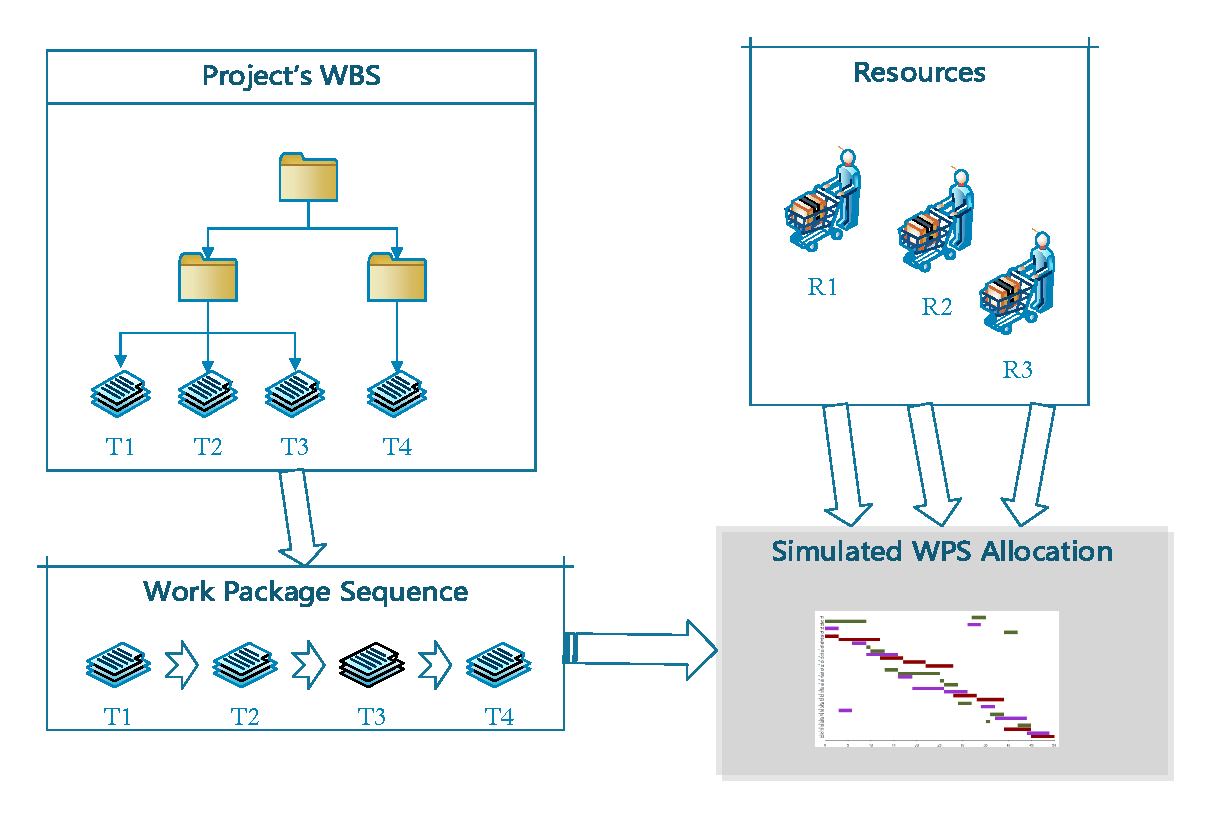
\includegraphics[width=0.8\textwidth]{figures/simu.pdf}
%%   \caption{Project Plan of Software Development}
%%   \label{fig:simu}
%% \end{figure}

%% There are two important steps in using the evolutionary algorithm. One is to
%% choose the representation of the problem's solution, the other is to define a
%% appropriate fitness function. In the process of project management, the work
%% packages in the project are allocated by simulation. See figure \ref{fig:simu},
%% Firstly, the whole project is decomposed into several work packages by
%% \emph{work breakdown structure}, and those work packages are arranged into a
%% corresponding \emph{work package sequence}. Secondly, according to the
%% dependencies of the work packages and the restriction of resource, each kinds of
%% resources is allocated to the corresponding work package by
%% \emph{first-come-first-served} algorithm. Finally, the project's overall
%% duration is calculate by simulation.


\subsection{The Representation of Solution}
%
For the above-mentioned problem, the representation of solution is defined as
follows.


This paper uses \emph{work package sequence} (hereinafter referred to as \emph{WPS}) to
represent a solution of project management problem. The representation of such a
solution is actually a priority arrangement sequence of the work packages in
the whole project, and the number of solutions for a project containing the $N$
work packages is $N!$, which is large enough to do random search.

%This is a figure 7
\begin{equation}
  T_1 \rightarrow T_5 \rightarrow T_6 \rightarrow T_4 \rightarrow T_8
  \rightarrow T_3 \rightarrow T_9 \rightarrow T_2 \rightarrow T_7
  \label{repr}
\end{equation}

For example, equation (\ref{repr}) is solution, the solution represents the work
package sequence in the priority of $T_1$, $T_5$, $T_6$, $T_4$, $T_8$, $T_3$,
$T_9$, $T_2$, $T_7$, while arranging the work packages. This representation is
beneficial and intuitive to programming.


\subsection{Fitness Evaluation}
%
The above-mentioned representation of solution make each individual coded as
\emph{WPS}. The fitness value of \emph{WPS} is the project's overall duration,
which is calculated by simulating the assignment of work packages in the set of
package sequence, see equation (\ref{wps}).

For each \emph{WPS}, the algorithm to calculate corresponding project overall
duration is as follows. Firstly, according to first-come-first-served (FCFS)
rule, the front work packages in a \emph{WPS} have high priority to get
resources, the back work packages has low priority. Secondly, the $TR$ function
defines which work package can get which resources, if two work packages that
require the same resources, the higher priority one will use the resources
firstly, the lower priority one will use the resources after the higher one
releases the resources. Finally, the project's overall duration is the last end
time after all work packages are allocated the resources (see algorithm
\ref{alg}).


\begin{algorithm}
  \caption{Fitness Evaluation Algorithm}
  \label{alg}
  \begin{algorithmic}
    \REQUIRE $WPS, R, TE, TR$
    \ENSURE $duration$
    \FOR {$i$ \textbf{from} $1$ \textbf{to} $WPS.length$}
      \STATE $t \gets WPS[i]$
      \STATE $ effort \gets TE(i)$
      \FOR {$r$ \textbf{in} $R$}
        \STATE $r.occupy \gets 0$
      \ENDFOR 
      \FOR {$r$ \textbf{in} $R$}
        \IF{$TR(t,r) = true$}
          \STATE $t.start \gets r.occupy$
          \STATE $t.end \gets r.occupy + effort$
          \STATE $r.occupy \gets t.end$
          \STATE \textbf{break}
        \ENDIF
      \ENDFOR
    \ENDFOR
    \STATE $duration \gets 0$  
    \FOR {$t$ \textbf{in} $WPS$}
      \IF{$t.end > duration$}
        \STATE $duration \gets t.end$
      \ENDIF
    \ENDFOR
  \end{algorithmic}
\end{algorithm}

\subsection{Genetic Operators}
%

There are two main types of operators in evolutionary algorithms:
\emph{crossover} and \emph{mutation}.

\subsubsection{Crossover}
In evolutionary algorithms, crossover is a genetic operator used to vary the
programming of a chromosome or chromosomes from one generation to the next.  In
this paper, we use a two-point crossover,that is , two points is selected
randomly on the parent organism strings. Everything between the two points is
swapped between the parent organisms, rendering two child organisms then
exchange corresponding part of chromosomes to get offspring individual.


\subsubsection{Mutation}
In evolutionary algorithms, Mutation is a genetic operator used to maintain
genetic diversity from one generation of a population of genetic algorithm
chromosomes to the next.  In this paper, we use two-point exchange mutation,
that is, two points is selected randomly on individual organisms strings, and
then exchange the two points.


\subsection{Parallel Evolutionary Algorithm}
%
Figure \ref{fig:flow} summarizes the basic process of the evolutionary
algorithm.


\begin{figure}[!ht]
  \centering
  % fisrt figure
  \begin{minipage}{0.40\textwidth}
    \centering
    \subfigure[Sequential] {
      \label{fig:flow:s}
      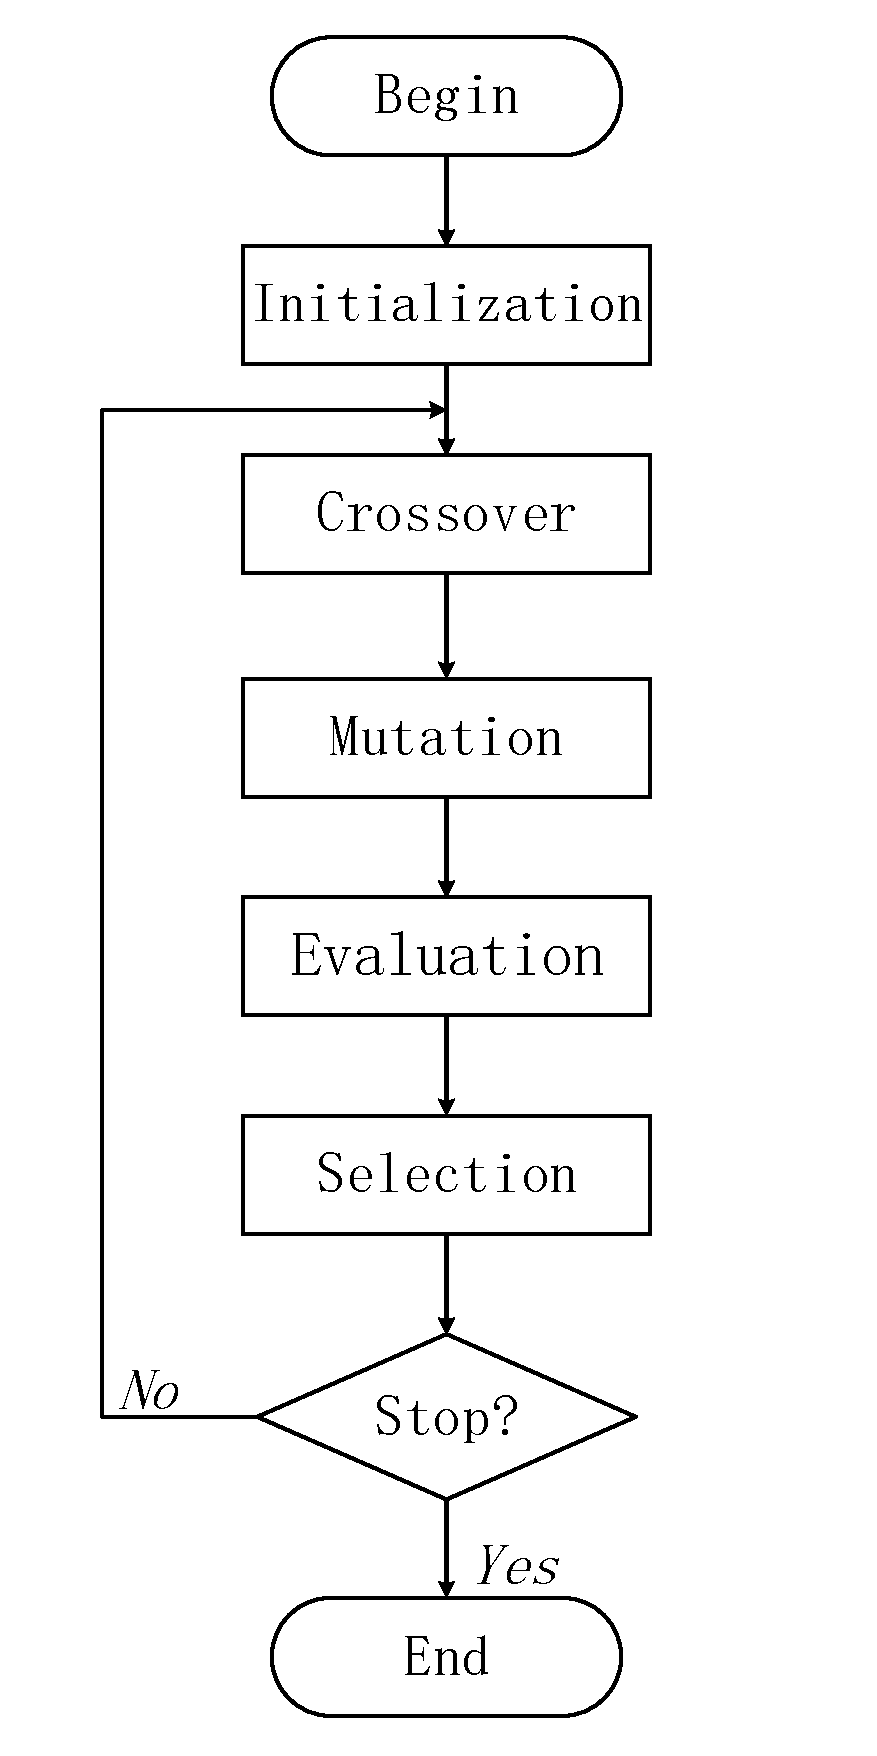
\includegraphics[width=\textwidth]{figures/ea_flow.pdf}
    }
  \end{minipage}
  % second figure
  \begin{minipage}{0.58\textwidth}
    \centering
    \subfigure[Parallel] {
      \label{fig:flow:p}
      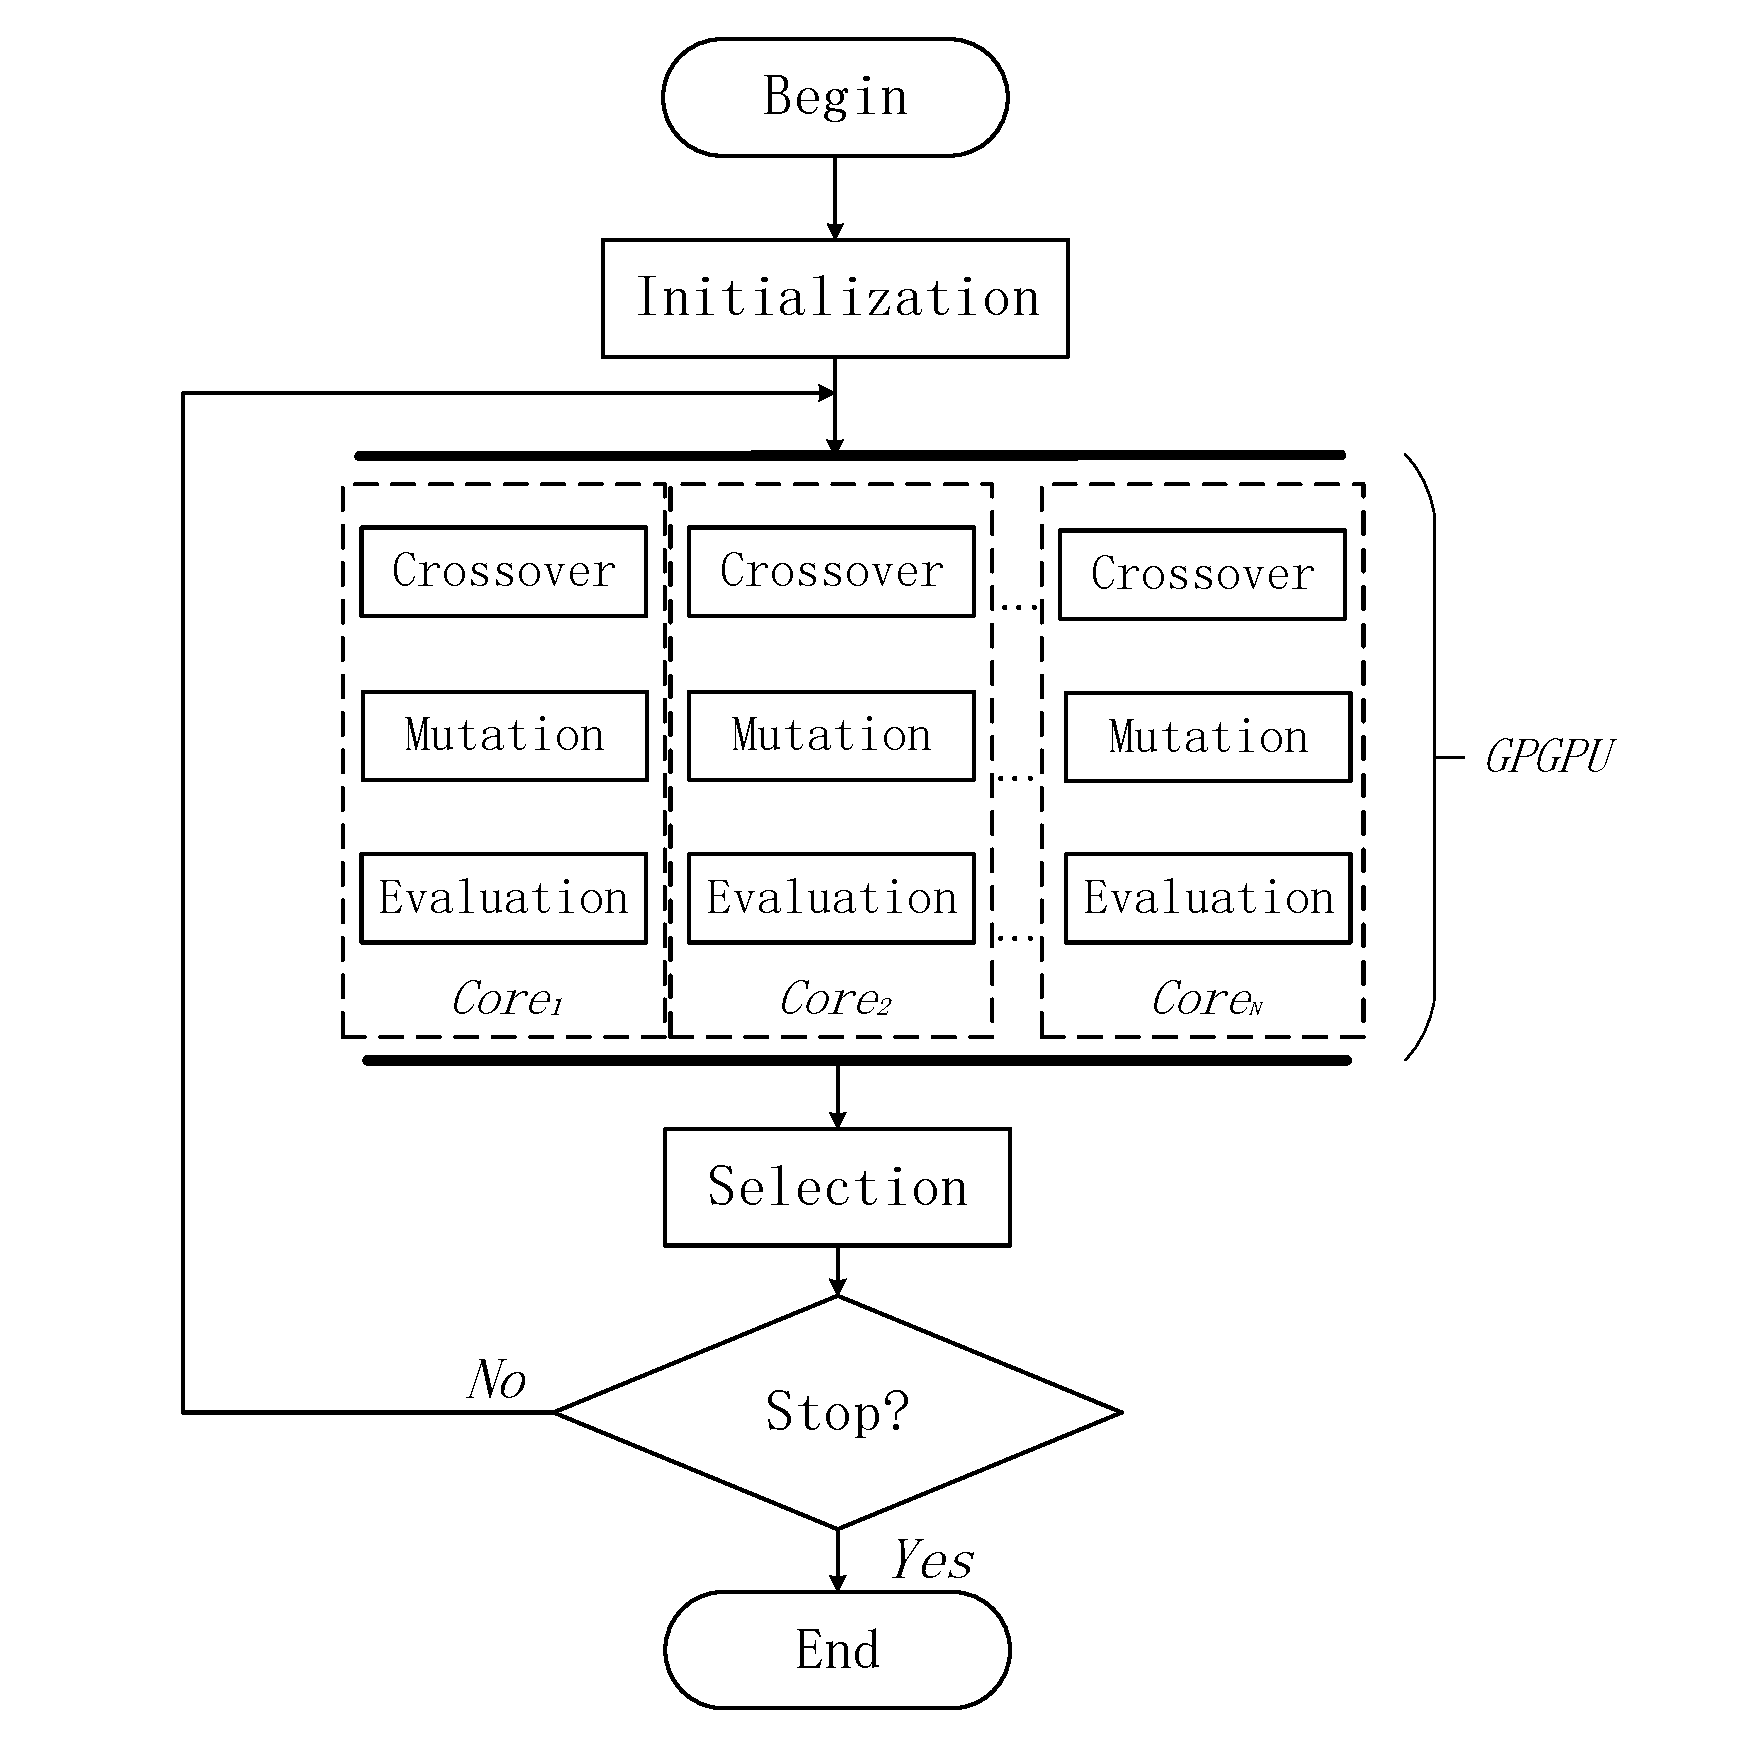
\includegraphics[width=\textwidth]{figures/ea2_flow.pdf}
    }
  \end{minipage}
  \caption{Sequential and Parallel Evolutionary Algorithm}
  \label{fig:flow}
\end{figure}


Figure \ref{fig:flow:s} is common sequenctial evolutionary algorithm, the
algorithm have several steps, such as initialization, crossover, mutation, and
selection. Candidate solutions to the optimization problem play the role of
individuals in a population, and the fitness function determines the convergence
of the solutions. Evolution of the population then takes place after the
repeated application of the above operators.


Figure \ref{fig:flow:p} illustrates a parallel evolutionary algorithm. The
parallel one follows most steps in sequenctial one, but put the top
time-consuming work on GPU. The steps of crossover, mutation and evolution runs
in different cores in GPU so that the speed of calculation can be impoved a lot.




\section{Evaluation}
%
text

%
% ---- Bibliography ----
%
\begin{thebibliography}{}
%
\bibitem[1]{stellman}
A. Stellman, and J. Greene.:
Applied Software Project Management.
OREILLY, (2005)

\bibitem[2]{chang}
C. K. Chang, H. Jiang, Y. Di, D. Zhu, and Y. Ge.:
Time-line Based Model for Software Project 
Scheduling with Genetic Algorithms.
Information and Software Technology, 1142-1154 (2008)

\bibitem[3]{alba}
E. Alba, and C. J. Francisco.:
Software Project Management with GA.
Information Sciences, 2380-2401 (2007)

\bibitem[4]{ren}
J. Ren, M. Harman, and M. D. Penta.:
Cooperative Co-evolutionary Optimization of Software 
Project Staff Assignments and Job Scheduling.
Lecture Notes in Computer Science, Springer Berlin Heidelberg, 495-519 (2011)

\bibitem[5]{pentico}
D. W. Pentico.:
Assignment Problems: A Golden Anniversary Survey.
European Journal of Operational Research, 774-793 (2007)

\bibitem[6]{penta}
M. D. Penta, M. Harman, and G. Antoniol.:
The Use of Search-based Optimization Techniques to 
Schedule and Staff Software Projects: An Approach and an Empirical Study. 
Software: Practice and Experience, 495-519 (2011)

\bibitem[7]{pospichal}
P. Pospichal, J. Jaros, and J.:
Schwarz. Parallel Genetic Algorithm on the CUDA Architecture.
Lecture Notes Computation Science, 442-451 (2010)

% \bibitem[8]{qu}
% 曲婉玲, 刘田.:
% 算法设计与分析.
% 北京:清华大学出版社, 205-207 (2011)

\bibitem[9]{stylianou}
C. Stylianou, S. Gerasimou, and A. S. Andreou.:
A Novel Prototype Tool for Intelligent Software 
Project Scheduling and Staffing Enhanced with Personality Factors.
IEEE 24th International Conference on Tools with Artificial Intelligence. 277-284 (2012)

\bibitem[10]{samanta}
S. Samanta.:
Genetic Algorithm: An Approach for Optimization (Using MATLAB). 
International Journal of Latest Trends in Engineering and Technology, 261-267 (2014)

\bibitem[11]{holland}
J. H. Holland.:
Adaptation in Natural and Artificial Systems: an Introductory 
Analysis with Applications to Biology, Control, and Artificial Intelligence.
U Michigan Press, (1975)

\bibitem[12]{harman}
M. Harman, P. McMinn, J. T. D. Souza, and S. Yoo.:
Search Based Software Engineering: Techniques, Taxonomy, Tutorial.
Empirical software engineering and verification, 1-59 (2012)

\bibitem[13]{deb}
K. Deb, A. Pratap, S. Agarwal, and T. Meyarivan.:
A Fast and Elitist Multiobjective Genetic Algorithm: NSGA-II.
IEEE Transactions on Evolutionary Computation, 182-197 (2002)

\bibitem[14]{vidal}
P. Vidal, and E. Alba.:
A Multi-GPU Implementation of a Cellular Genetic Algorithm.
2010 IEEE World Congress on Computational Intelligence, 1-7 (2010)

% \bibitem[15]{kirk}
% D.B. Kirk, W. W. Hwu.:
% 大规模并行处理器编程实战(第二版).
% 北京: 清华大学出版社, 1-31 (2013)




% ---------------------------------
% \bibitem[1980]{2clar:eke}
% Clarke, F., Ekeland, I.:
% Nonlinear oscillations and
% boundary-value problems for Hamiltonian systems.
% Arch. Rat. Mech. Anal. 78, 315--333 (1982)

% \bibitem[1981]{2clar:eke:2}
% Clarke, F., Ekeland, I.:
% Solutions p\'{e}riodiques, du
% p\'{e}riode donn\'{e}e, des \'{e}quations hamiltoniennes.
% Note CRAS Paris 287, 1013--1015 (1978)

% \bibitem[1982]{2mich:tar}
% Michalek, R., Tarantello, G.:
% Subharmonic solutions with prescribed minimal
% period for nonautonomous Hamiltonian systems.
% J. Diff. Eq. 72, 28--55 (1988)

% \bibitem[1983]{2tar}
% Tarantello, G.:
% Subharmonic solutions for Hamiltonian
% systems via a $\bbbz_{p}$ pseudoindex theory.
% Annali di Matematica Pura (to appear)

% \bibitem[1985]{2rab}
% Rabinowitz, P.:
% On subharmonic solutions of a Hamiltonian system.
% Comm. Pure Appl. Math. 33, 609--633 (1980)

\end{thebibliography}
\clearpage

% end of bibliography


\end{document}
